\section{Feasibility: land, demand, and orbit}
\label{sec:feasibility}

\paragraph{How little land it takes.} We apply a deliberately conservative
``do no ecological harm'' filter: eligible land is barren desert (only a
$20\%$ usable slice, excluding dunes, reserves, and remote terrain) plus
rooftops on built-up land. That leaves \DeployableMkm~million~km$^2$. At
$20\%$ module efficiency and an $0.8$ performance ratio on desert-grade
irradiance, this deployable footprint delivers \DeployableTW~TW on
average --- about \TimesElec$\times$ world electricity demand and
\TimesPrimary$\times$ total primary energy (Figure~\ref{fig:land}). Inverting
the calculation, all of world electricity fits on \AreaWorldKm~km$^2$ of
panel: a single square roughly \AreaWorldSide~km on a side. The potential is
simply not the bottleneck.

\begin{figure}[t]
\centering
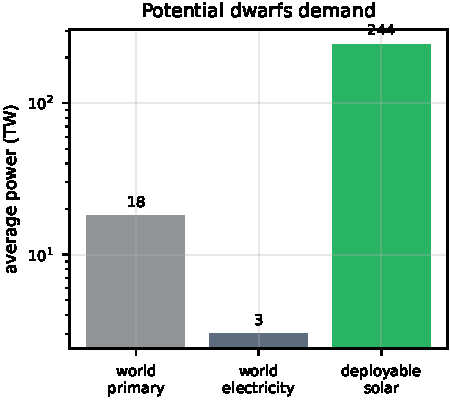
\includegraphics[width=0.85\linewidth]{figures/land_vs_demand.pdf}
\caption{Average power (log scale): world primary energy and electricity
demand against the deployable desert-and-rooftop solar resource. Potential
exceeds demand by more than an order of magnitude.}
\label{fig:land}
\end{figure}

\paragraph{The orbital alternative.} If land or intermittency were the
constraint, a collector in orbit --- a ``layer'' catching sunlight above the
atmosphere --- is the natural escape, and a modest cousin of a Dyson sphere.
Our chain accounting (Figure~\ref{fig:sbsp}) puts the delivered power at
\SpaceWm~W per m$^2$ of collector versus \GroundWm~W per m$^2$ of desert panel,
a \SbspRatio$\times$ advantage. Crucially, the advantage is \emph{not} mainly
from avoiding atmospheric absorption: microwave downlink already passes the
atmosphere at $\sim\!95\%$. It comes from the capacity factor --- an orbital
collector sees the Sun \SpaceCF\% of the time at full strength, versus an
effective \GroundCF\% on the ground once night and weather are counted. The
conversion and transmission chain (PV, DC-to-RF, downlink, rectenna) gives back
much of that gain, so orbit is a capacity-factor play, not a free-energy one.

\begin{figure}[t]
\centering
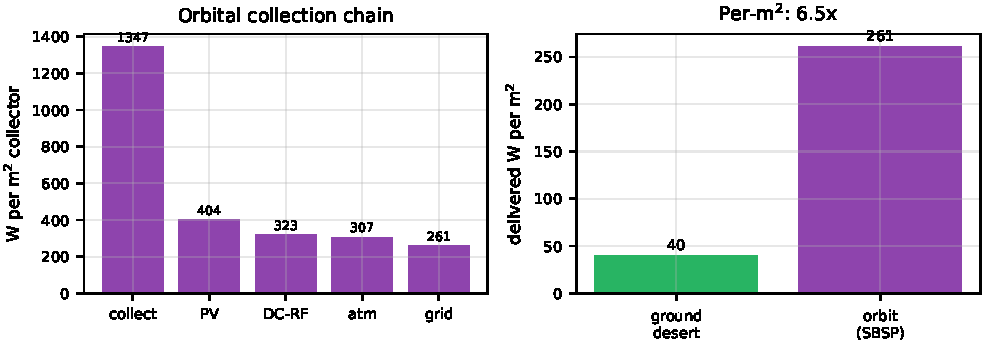
\includegraphics[width=\linewidth]{figures/sbsp.pdf}
\caption{\textbf{Left:} orbital collection-to-grid chain, W per m$^2$ of
collector. \textbf{Right:} delivered power per m$^2$, ground desert panel vs
space-based (\SbspRatio$\times$).}
\label{fig:sbsp}
\end{figure}
